\begin{appendices}

\addtocontents{toc}{\protect\renewcommand{\protect\cftchappresnum}{\appendixname\space}}
\addtocontents{toc}{\protect\renewcommand{\protect\cftchapnumwidth}{7em}}

%%%%%%%%%%%%%%%%%%%%%%%%%%%%%%%%%

\chapter{Instabilities of the homogeneous state}

\label{sec:phasesep}

We briefly examine the stability of the homogeneous state when it is introduced in the two regimes from \figref{fig:free_energy}, namely the nucleation and growth regime and the spinodal decomposition regime, and prove that a necessary condition for spontaneous phase separation is $f''(\phi) < 0$, i.e. regions where $f(\phi)$ is convex.
Here $f(\phi)$ is the free energy density given by \Eqref{eqn:free_energy_formulation} or \Eqref{eqn:free_energy}, as both of the free energy densities exhibit identical behaviour for stability of the phases; see Ref. \cite{Review2019}.

\section{Spinodal decomposition regime}

We first focus on the spinodal decomposition regime, where infinitesimal fluctuations in the homogeneous state are unstable, thus promoting phase separation into the minima described by the free energy density. 
We start by assuming in an homogeneous state, small perturbations lead to the formation of two phase separated domains, each of volume $\delta V$.
The resulting volume fractions for the two domains read as $\phi_1 = \phi - \delta \phi$ and $\phi_2 = \phi + \delta \phi$, as mass conservation dictates that the average volume fraction $\phi$ must remain constant.
The free energy change in this case can be calculated as: 
\begin{equation*}
    \delta F = \delta V f(\phi_1) + \delta V f(\phi_2) - 2 \delta V f(\phi) = \delta V (\delta \phi)^2 f''(\phi).
\end{equation*}
Thus, we see that if $f''(\phi) < 0$ (i.e. $f(\phi)$ is convex), the infinitesimal perturbations are energetically favourable and will grow.
This regime is commonly referred to as the Spinodal decomposition; see \figref{fig:free_energy}.
Consequently,  $f''(\phi) > 0$ implies that the perturbations will die down, making phase separation energetically unfavourable for infinitesimal perturbations.
We will now see the conditions for phase separation to be initiated in the region where $f(\phi)$ is concave. 

\section{Nucleation and growth regime}

We now focus on the nucleation and growth regime and see the conditions for which the perturbations in this regime grow.
As infinitesimal perturbations in this regime die down quickly, we explore what happens when we have finite perturbations.

Let us assume the finite perturbation to be of the kind where a droplet of radius $R$ forms and the volume fraction in the dilute phase $\phiOut$ changes by an amount $\delta \phi$, where $\delta \phi \ll \phi$.
From \Eqref{eqn:constraint_3}, the free energy change in this case can be calculated as: 
\begin{equation}
\label{eqn:infinitesimal_change_0}
    \delta F = V_d f(\phiIn) + (V - V_d) f(\phi - \delta \phi) - V f(\overline{\phi}) + S \gamma,
\end{equation}
where we used $\phiOut = \phi - \delta \phi$, $V$ is the volume of the system, $V_d = (4/3) \pi R^3$ is the volume of the droplet, $S = 4 \pi R^2$ is the surface area and $\overline{\phi}$ is the average volume fraction. 
Similarly, from \Eqref{eqn:constraint_4}, we have $V_d \, \phiIn + (V - V_d) (\phi - \delta \phi) = V \overline{\phi}$.
Thus, we calculate the change in volume fraction $\delta \phi$ as:
\begin{equation}
\label{eqn:infinitesimal_change_1}
    \delta \phi = \phi - \frac{V \overline{\phi} - V_d \phiIn}{V - V_d}.
\end{equation}
Expanding $\delta \phi$ from \Eqref{eqn:infinitesimal_change_1} in linear order, we have from \Eqref{eqn:infinitesimal_change_0},
\begin{equation}
\label{eqn:infinitesimal_change_2}
    \delta F \approx V_d [f(\phiIn) - f(\phi) - f'(\phi)(\phiIn - \phi)] + S \gamma.
\end{equation}
From \Eqref{eqn:infinitesimal_change_2}, we can qualitatively see that the term $S \gamma \, (\sim R^2)$ will dominate for small radius and thus increasing the droplet radius further is not energetically favourable. 
On the other hand for large radius, the term proportional to $V_d$ will dominate ($\sim R^3$). 
Hence, if the droplet is larger than a critical radius $R_c$, it will further lower the free energy as it increases in size.
We can calculate this critical radius by setting $\partial_R\,\delta F = 0$, which gives us:
\begin{equation*}
    R_c = (2 \gamma) / [f(\phiIn) - f(\phi) - f'(\phi)(\phiIn - \phi)].
\end{equation*}
Note that the critical radius $R_c$ is proportional to the surface tension $\gamma$.
We hence prove that in the nucleation and growth regime, sufficiently finite perturbations are required to initiate phase separation and form droplets. 

%%%%%%%%%%%%%%%%%%%%%%%%%%%%%%%%%

\chapter{Droplet dynamics for spherical droplets}

\label{sec:droplet_dynamics}

Here, we derive the equations for the growth speed and drift rate of droplets of arbitrary shape described by \Eqsref{eqn:droplet_dynamics} in two and three dimensions; see Refs. \cite{Review2019,Weber2017}.
% The general shape of a droplet is described by its surface $\Omega$.
% Assuming that the 2 dimensional surface of a 3 dimensional droplet (and correspondingly the 1 dimensional curve of a 2 dimensional droplet) does not deviate a lot from it's spherical shape, we place a spherical co-ordinate system centered on the droplet in 3 dimensions (and a polar co-ordinate system in 2 dimensions).

% The position vector of the droplet surface can be defined as $\vec{R}(\theta, \varphi,t) = P(\theta, \varphi,t) \, \vec{e}_{\mathrm{r}}$ in 3 dimensions and $\vec{R}(\theta, t) = P(\theta,t) \, \vec{e}_{\mathrm{r}}$ in 2 dimensions, where $P$ is the surface parameterization of the droplet surface at time $t$.
% The interfacial velocity $\vec{v}$ can then be split into radial and normal components to the droplet surface as $v_\mathrm{n}$ and $v_\mathrm{r}$.
% From geometry, it follows that $v_\mathrm{r} ~ \vec{e}_\mathrm{r} \cdot \vec{n} = v_\mathrm{n}$, where $\vec{r}, \vec{n}$ are the interfacial velocities in the outward radial and normal directions respectively.

% Droplet growth rate follows from rate of change of volume of the droplet, which we calculate next. 
% The volume of the drop is defined as:
% \begin{subequations}
% \begin{align}
%     V_\mathrm{3D} &=\int_{\theta} \int_{\varphi} \int_{r}  \, r^2 \sin\theta \,  \mathrm{d}\theta  \, \mathrm{d}\varphi \,  \mathrm{d}r = (1 / 3) \int_{\theta} \int_{\varphi} P(\theta, \varphi, t)^3 \, \sin\theta \,  \mathrm{d}\theta  \, \mathrm{d}\varphi \nonumber \mathrm{~and~}
%     \\[10pt]
%     V_\mathrm{2D} &= \int_{\theta} \int_{r} r\,\mathrm{d}r \, \mathrm{d}\theta = (1 / 2) \int_{\theta} P(\theta, t)^2 \,\mathrm{d}\theta, \nonumber
% \end{align}
% \end{subequations}
% where, throughout this section, the subscripts $\mathrm{2D/3D}$ indicate in 2 dimensions and in 3 dimensions respectively. 
% The rate of volume change reads as:
% \begin{subequations}
% \begin{align}
%     \partial_t V_\mathrm{3D} &= \int_{\theta} \int_{\varphi} P(\theta, \varphi, t)^2  \, \partial_t P(\theta, \varphi, t) \,  \sin\theta \,  \mathrm{d}\theta \,  \mathrm{d}\varphi \nonumber \mathrm{~and~}
% 	\\[10pt]
% 	\partial_t V_\mathrm{2D} &= \int_{\theta} P(\theta, t) \,  \partial_t P(\theta, t) \,\mathrm{d}\theta. \nonumber
% \end{align}
% \end{subequations}

% % Alternatively, we also note that $\partial_t V_\mathrm{2D/3D} = S_\mathrm{2D/3D}~\partial_t M_\mathrm{2D/3D}$, where $S_\mathrm{2D/3D}$ is the surface area of the droplet and $M_\mathrm{2D/3D}$ is the volume averaged radius of the droplet at time $t$ in 2 and 3 dimensions respectively.

% Alternatively, we also note that $\partial_t V_\mathrm{2D/3D} = S_\mathrm{2D/3D}~\partial_t M_\mathrm{2D/3D}$, where $S_\mathrm{2D/3D}$ is the surface area of the droplet and $M_\mathrm{2D/3D}$ is the volume averaged radius of the droplet in 2 and 3 dimensions respectively.
% Equating the two expressions for $\partial_t V_\mathrm{2D/3D}$, we have:
% \begin{subequations}
% \begin{align}
%     \partial_t M_\mathrm{3D} &= S^{\,-1}_\mathrm{3D} \,  \int_{\theta} \int_{\varphi} P(\theta, \varphi, t)^2  ~ \partial_t P(\theta, \varphi, t) \,  \sin\theta \,  \mathrm{d} \theta \,  \mathrm{d}\varphi \nonumber \mathrm{~and~}
% 	\\[10pt]
%     \partial_t M_\mathrm{2D} &= S^{\,-1}_\mathrm{2D} \, \int_{\theta} P(\theta, t) ~  \partial_t P(\theta, t) \,\mathrm{d}\theta. \nonumber
% \end{align}
% \end{subequations}
% Finally, assuming a spherical droplet at all times, i.e. $P(\theta, \varphi, t) = M_\mathrm{3D}$ and $P(\theta, t) = M_\mathrm{2D}$, we have:
% \begin{subequations}
% \begin{align}
%     \partial_t M_\mathrm{3D} &= (1 / 4 \pi) \int_{\theta} \int_{\varphi} \partial_t P(\theta, \varphi, t) \,  \sin\theta \,  \mathrm{d}\theta \, \mathrm{d}\varphi \nonumber \mathrm{~and~}
% 	\\[10pt]
%     \partial_t M_\mathrm{2D} &= (1 / 2 \pi) \int_{\theta} \partial_t P(\theta, t) \,  \mathrm{d}\theta, \nonumber
% \end{align}
% \end{subequations}
% which in fact becomes \Eqref{eqn:DropletGrowth} when the integral is considered over the droplet surface.

% Furthermore, the centroid of the droplet can be calculated as:
% \begin{subequations}
% \begin{align}
%     C_\mathrm{3D} &= \left[\int_{\theta}\int_{\varphi}\int_{r} \,  (r^2 \,  \sin\theta \,  \mathrm{d}\theta \,  \mathrm{d}\varphi \, \mathrm{d}r )  \, ( r \, \vec{e_p} \cdot \vec{e_r}) \right] \bigg/ \left[\int_{\theta} \int_{\varphi} \int_{r} \mathrm{d} V_\mathrm{3D} \right] \nonumber \mathrm{~and~}
% 	\\[10pt]
%     C_\mathrm{2D} &= \left[\int_{\theta} \int_{r} (r\,\mathrm{d}r \, \mathrm{d}\theta) \, (r \, \vec{e_p} \cdot \vec{e_r}) \right] \bigg/ \left[\int_{\theta} \int_{r} \mathrm{d} V_\mathrm{2D}\right], \nonumber
% \end{align}
% \end{subequations}
% where $\vec{e_p}$ is the co-ordinate along which calculating the centroid is desired.
% Following the same procedure used to calculate rate of volume change, we obtain the droplet drift speed as:
% \begin{subequations}
% \begin{align}
%     \partial_t C_\mathrm{3D} &= V^{\,-1}_\mathrm{3D} \int_{\theta} \int_{\varphi} P(\theta, \varphi, t)^3 ~ \partial_t P(\theta, \varphi, t)  \, \vec{e_p} \cdot \vec{e_r} \, \sin\theta \mathrm{d} \theta \,  \mathrm{d}\varphi \nonumber \mathrm{~and~}
% 	\\[10pt]
%     \partial_t C_\mathrm{2D} &= V^{\,-1}_\mathrm{2D} \int_{\theta} P(\theta, t)^2  ~  \partial_t P(\theta, t) \, \vec{e_p} \cdot \vec{e_r} \, \mathrm{d} \theta. \nonumber
% \end{align}
% \end{subequations}

% Hence, we get
% \begin{subequations}
% \begin{align}
%     \partial_t C_\mathrm{3D} &= (3 / 4 \pi) \int_{\theta} \int_{\varphi} \partial_t P(\theta, \varphi, t) \, \vec{e_p} \cdot \vec{e_r} \, \sin\theta \,  \mathrm{d} \theta \,  \mathrm{d}\varphi \nonumber \mathrm{~and~}
% 	\\[10pt]
%     \partial_t C_\mathrm{2D} &= (1 / \pi) \, \int_{\theta} \partial_t P(\theta, t)  \, \vec{e_p} \cdot \vec{e_r} \, \mathrm{d} \theta, \nonumber
% \end{align}
% \end{subequations}
% which becomes \Eqref{eqn:DropletDrift} when the integral is evaluated over the surface of the droplet in 2 and 3 dimensions, and we arrive at \Eqsref{eqn:droplet_dynamics} describing droplet dynamics.
For simplicity, we focus on $d=3$ dimensions, but the derivation works analogously in all dimensions.
The 2D surface of a 3D droplet can be parameterized by points $\vec{R}(\theta, \varphi)$ with parameters $\theta$ and $\varphi$.
For simplicity, we consider droplet shapes that are star domains, so we can place a spherical coordinate system inside the droplet and write $\vec{R}(\theta, \varphi,t) = P(\theta, \varphi, t)  \vec{e}_r$, where $\theta$ and $\varphi$ denote the typical angles and $P(\theta, \varphi, t)$ denotes the distance of the surface from the origin.

The droplet volume reads $V = d^{-1} \int P^d \, \diff\Omega$, where $\diff\Omega$ is the solid angle element, which reads $\diff\Omega = \sin\theta \, \diff\theta\diff\varphi$ for spherical coordinates.
The volume changes in time as $\partial_t V = \int (\partial_t P) \, P^{d-1} \, \diff\Omega$, where $\partial_t P$ is the interfacial speed in the radial direction.
We obtain it from the normal speed $v_\mathrm{n}$, given by \Eqref{eqn:InterfacialSpeed}, using the geometric relation $v_\mathrm{n} = (\partial_t P) \, \vec{e}_r \cdot \vec{n}$, which implies $\partial_t P = v_\mathrm{n} / (\vec{e}_r \cdot \vec{n})$.

Additionally, the differential element~$\diff\Omega$ can be linked to the surface area element~$\diff A$ by $P^{d-1}\diff\Omega = \vec{e}_r \cdot \vec{n} \, \diff A$.
Taken together, the rate of change of the radius~$R$ of a sphere with volume~$V$, given by $\partial_t R = (\partial_t V)/S$ for the surface area~$S$, can then be expressed as  \Eqref{eqn:DropletGrowth}.

Similarly, we analyze the center-of-mass position $\vec x = [(d+1)V]^{-1} \int P^{d+1} \vec{e}_r \diff\Omega$.
We find $\partial_t(\vec x V) = \int \! P^d (\partial_t P) \vec{e}_r \diff\Omega = \int \! P v_\mathrm{n} \vec{e}_r \, \diff A$.
If the droplet is initially centered on the origin, $\vec x =0$, this implies  $\partial_t \vec x = V^{-1}\int \! P v_\mathrm{n} \vec{e}_r\, \diff A$.
This expression is equivalent to \Eqref{eqn:DropletDrift} for spherical droplets, where $P(\theta, \varphi)=R$, $\vec{e}_r=\vec{n}$, and $R/V = d/S$.

%%%%%%%%%%%%%%%%%%%%%%%%%%%%%%%%%
\chapter{Interfacial velocity of droplets}

\label{sec:interfacial_speed_derivation}

Here, we briefly derive the interfacial speed of the droplets.  
We investigate the dynamics of the droplet interface by analyzing an infinitesimal cuboid placed on the interface.
The cuboid is aligned with the interface and covers an area element~$\diff A$ of it.
It protrudes by distances $\epsilon_\mathrm{in}$ and $\epsilon_\mathrm{out}$ inside and outside the interface, respectively, so its volume is given by $(\epsilon_\mathrm{in} + \epsilon_\mathrm{out}) \, \diff A$.

Keeping the cuboid fixed in space, the distances change by the interfacial speed $v_\mathrm{n}$ in the normal direction, $\partial_t \epsilon_\mathrm{in} = - \partial_t \epsilon_\mathrm{out} = v_\mathrm{n}$.
We use this to express the time derivative of the amount of material in the cuboid, $\Phi = ( \epsilon_\mathrm{in} \phiEqIn + \epsilon_\mathrm{out} \phiEqOut )\, \diff A$, as
%\begin{align}
%    \partial_t {\Phi} &= \bigl(
%    	\phiEqIn  \partial_t \epsilon_\mathrm{in} + \epsilon_\mathrm{in} \partial_t \phiEqIn
%	+  \phiEqOut \partial_t \epsilon_\mathrm{out}+  \epsilon_\mathrm{out} \partial_t \phiEqOut
%	\bigr) \, \diff A.
$    \partial_t {\Phi} = \bigl(
    	\phiEqIn v_\mathrm{n} + \epsilon_\mathrm{in} \partial_t \phiEqIn
	-  \phiEqOut v_\mathrm{n} +  \epsilon_\mathrm{out} \partial_t \phiEqOut
	\bigr) \diff A$.
%    \label{eqn:volume_change}
%\end{align}
On the other hand, the amount~$\Phi$ changes due to material fluxes, $\partial_t \Phi \approx ( \jIn - \jOut) \cdot \vec{n} \, \diff A$, where we neglect chemical reactions in the infinitesimal volume element and divergences of fluxes tangential to the interface.

Equating the two expressions for $\partial_t \Phi$ in the limit of vanishing $\epsilon_\mathrm{in}$ and $\epsilon_\mathrm{out}$, we have
\begin{equation*}
	\vn \approx \frac{\jIn - \jOut}{\phiEqIn - \phiEqOut} \cdot \vec{n},
\end{equation*}
which is \Eqref{eqn:InterfacialSpeed}.
We thus have an expression for the normal interfacial speed $v_\mathrm{n}$ in terms of the fluxes $\jIn, \, \jOut$.

%%%%%%%%%%%%%%%%%%%%%%%%%%%%%%%%%

\chapter{Fluxes evaluated inside the droplets}

\label{sec:fluxes_inside_droplets}

We seek to determine the fluxes $\jIn$ inside the droplet. As the fluxes follow from the volume fraction profile inside the droplet $\phiIn$, which is determined from the stationary state of \Eqsref{eqn:thin_interface_model} as:

\begin{equation*}
    \frac{\partial \phi_\mathrm{in}}{\partial t}
    \approx D_\mathrm{in} \nabla ^2 \phi_\mathrm{in} +
    s(\phi^{0}_\mathrm{in})
    - k_{\mathrm{in}}(\phi_\mathrm{in} - \phi^{0}_\mathrm{in}),
\end{equation*}
where $D_\mathrm{in} = \Lambda(\phi^0_\mathrm{in})\,b$ is diffusivity.
We solve the steady state of above equation for $\phiIn$ in a co-ordinate system with angular symmetry centered at the droplet.
We use the boundary conditions $\phi_\mathrm{in}(R) = \phiEq_\mathrm{in}$ and $\partial_r \phi_\mathrm{in}(0) = 0$, where $r$ is the radial co-ordinate. 
$\phiIn$ then reads in 1, 2 and 3 dimensions as
\begin{subequations}
\label{eqn:fluxes_outside_appendix}
\begin{align}
    \phi_\mathrm{in,3 \mathrm{D}}(r) &= \phi^0_\mathrm{in} + \frac{s(\phi^0_\mathrm{in})}{k_\mathrm{in}} - \frac{R\,\sinh \left(\frac{r}{\xi_\mathrm{in} }\right) s(\phiEqIn)}{r\ \text{sinh}\left(\frac{R}{\xi_\mathrm{in}}\right) k_\mathrm{in}},
    \\[10pt]
    \phi_\mathrm{in,2 \mathrm{D}}(r) &= \phi^0_\mathrm{in} + \frac{s(\phi^0_\mathrm{in})}{k_\mathrm{in}} - \frac{ I_0\left(\frac{r}{\xi_\mathrm{in} }\right) s(\phiEqIn)}{I_0\left(\frac{R}{\xi_\mathrm{in} }\right) k_\mathrm{in} },
    \\[10pt]
    \phi_\mathrm{in,1 \mathrm{D}}(r) &= \phi^0_\mathrm{in} + \frac{s(\phi^0_\mathrm{in})}{k_\mathrm{in}} - \frac{\cosh \left(\frac{r}{\xi_\mathrm{in} }\right) s(\phiEqIn)}{\text{cosh}\left(\frac{R}{\xi_\mathrm{in} }\right) k_\mathrm{in} },
\end{align}
\end{subequations}
where $I_0$ is the Modified Bessel Functions of the First Kind and $\xi_\mathrm{in} = \sqrt{D_\mathrm{in}/|k_\mathrm{in}|}$ is the reaction-diffusion length-scale; see Ref. \cite{Review2019}.
Assuming $R \ll \xi_\mathrm{in}$,
the fluxes inside the interface then read as \begin{equation}
    \vec{j}_\mathrm{in} \approx [-D_\mathrm{in} {\boldsymbol{\nabla}} \phi_\mathrm{in}(R)] \approx \frac{R}{d} \left [ s(\phi^{0}_\mathrm{in})
    - k_{\mathrm{in}}(\phi^\mathrm{eq}_\mathrm{in} - \phi^{0}_\mathrm{in}) \right ] \,\vec{n},
\end{equation}
where $d$ is the space dimension.

%%%%%%%%%%%%%%%%%%%%%%%%%%%%%%%%%

\chapter{Fluxes evaluated inside droplet shells}

\label{sec:fluxes_inside_shell}

We seek to determine the fluxes outside the droplet. 
The fluxes follow from the volume fraction profile outside the droplet $\phiOut$ by considering \Eqref{eqn:RD_dilute} in an annular shell of thickness\,$\ell$ surrounding the droplet, which we further discretize into $N$ sectors uniformly chosen in the angular dimensions; see Fig. \ref{fig:schematics}.

We assume the volume fraction in the $m$-th sector as $\phiOut^{(m)}(r)$ and solve for $\phiOut^{(m)}(r)$ using \Eqref{eqn:phi_out_in_shell} in stationary state along with the boundary conditions $\phiOut^{(m)}(R)=\phiEqOut$ and $\phiOut^{(m)}(R + \ell)= \phiShell^{(m)}$.
Here, we estimate $\phiShell^{(m)}$ from a linear interpolation of the discretized background field $\phi_\mathrm{out}$; see Fig. \ref{fig:schematics}.
Furthermore, we assume that $\phiOut^{(m)}(r)$ varies only marginally in the shell sector and we linearize the reaction flux $s(\phiOut^{(m)})$; see Ref. \cite{Review2019}, as 
\begin{equation*}
    s(\phiOut^{(m)}) \approx \Gamma_\mathrm{out} - \kOut\,\phiOut,
\end{equation*}
where $\Gamma_\mathrm{out}, \kOut$
are obtained from the constraints $s(\phiOut^{(m)})(R) = s(\phiEqOut)$ and $s(\phiOut^{(m)})(R + \ell) = s(\phiShell^{(m)})$; see \Eqsref{eqn:GammaOut_KOut}.
We can then evaluate the local material fluxes at the droplet surface in the normal direction as $\jOut^{(m)} \cdot \vec{n} = [-D_\mathrm{out} {\boldsymbol{\nabla}} \phiOut^{(m)}(R)] \cdot \vec{n} $, where $D_\mathrm{out}$ is the diffusivity outside the droplets.
The expressions for the normal fluxes in $1$, $2$, and $3$ dimensions read

\begin{subequations}
\label{eqn:FluxesOut_caseA}
\begin{align}
\begin{split}
    \vec{j}^{(m)}_\mathrm{out, 1D} \cdot \vec{n}
    &= D_\mathrm{out} \frac{(\phiEqOut \kOut - \Gamma_\mathrm{out}) \cosh \left(\frac{\ell}{\xi_\mathrm{out}}\right) -\left(\phiShell^{(m)} \kOut- \Gamma_\mathrm{out} \right) }{\kOut \xi_\mathrm{out} \sinh \left(\frac{\ell}{\xi_\mathrm{out} }\right)},
    \\[10pt]
    \vec{j}^{(m)}_\mathrm{out, 2D} \cdot \vec{n}
    &= D_\mathrm{out} \frac{
    (\phiEqOut \kOut-\Gamma_\mathrm{out})~T_1
	- \frac{\xi_\mathrm{out} }{R} \left(\phiShell^{(m)} \kOut - \Gamma_\mathrm{out}\right)
    }
    {\kOut \xi_\mathrm{out}~T_2},
    \\[10pt]
    \vec{j}^{(m)}_\mathrm{out, 3D} \cdot \vec{n}
    &=  D_\mathrm{out} \frac{(\phiEqOut \kOut - \Gamma_\mathrm{out}) \left(R \coth \left(\frac{\ell}{\xi_\mathrm{out} }\right) + \xi_\mathrm{out} \right)
	- \frac{\ell + R}{\sinh \left(\frac{\ell}{\xi_\mathrm{out} }\right)} \left( \phiShell^{(m)} \kOut - \Gamma_\mathrm{out}\right)
	} {\kOut \xi_\mathrm{out} R},
\end{split}
\end{align}
\end{subequations}
where $T_1,~T_2$ in $\vec{j}^{(m)}_\mathrm{out, 2D} \cdot \vec{n}$ are given by:
\begin{subequations}
\begin{align}
    T_1 &= \left[I_1\left(\frac{R}{\xi_\mathrm{out} }\right) K_0\left(\frac{\ell+R}{\xi_\mathrm{out} }\right) + K_1\left(\frac{R}{\xi_\mathrm{out} }\right) I_0\left(\frac{\ell+R}{\xi_\mathrm{out}}\right)\right] \nonumber
    \mathrm{~and~}
    \\[10pt]
    T_2 &= \left[K_0\left(\frac{R}{\xi_\mathrm{out} }\right) I_0\left(\frac{\ell+R}{\xi_\mathrm{out} }\right)-I_0\left(\frac{R}{\xi_\mathrm{out} }\right) K_0\left(\frac{\ell + R}{\xi_\mathrm{out} }\right)\right] \nonumber,
\end{align}
\end{subequations}
$K_\alpha, I_\alpha$ are Modified Bessel Functions of the Second and First Kind respectively, $R$ is the droplet radius, $\ell$ is the thickness of the shell sector and $\xi_\mathrm{out} = \sqrt{D_\mathrm{out}/|\kOut|}$ is the reaction-diffusion length-scale; see Ref. \cite{Review2019}.

Note that $\Gamma_\mathrm{out}, k_\mathrm{out}$ from \Eqsref{eqn:GammaOut_KOut} will diverge when $\phiShell^{(m)} \approx \phiEqOut$.
In that case, we reason that if $\phiShell^{(m)} \approx \phiEqOut$, $s(\phiShell^{(m)})$ will also be close to $s(\phiEqOut)$, as we consider linearized weak reactions.
We hence formulate $s(\phiOut^{(m)})$ as a constant value given by:
\begin{equation*}
    s(\phiOut^{(m)}) = \overline{\Gamma}_\mathrm{out} =  [s(\phiEqOut) + s(\phiShell^{(m)})] / 2.
\end{equation*}
The expressions for the normal fluxes in $1$, $2$, and $3$ dimensions then read
\begin{subequations}
\label{eqn:FluxesOut_caseB}
\begin{align}
    \vec{j}^{(m)}_\mathrm{out, 1D} \cdot \vec{n} 
    &= \frac{D_\mathrm{out} (\phiEqOut-\phiShell^{(m)})}{\ell}-\frac{\overline{\Gamma}_\mathrm{out} \ell}{2},
    \\[10pt]
    \vec{j}^{(m)}_\mathrm{out, 2D} \cdot \vec{n} 
    &= \frac{\overline{\Gamma}_\mathrm{out} \ell (\ell+2 R) - 4 \phiEqOut D_\mathrm{out} + 4 \phiShell^{(m)} D_\mathrm{out}}{4 R \log \left(\frac{R}{\ell+R}\right)}+\frac{\overline{\Gamma}_\mathrm{out} R}{2},
    \\[10pt]
    \vec{j}^{(m)}_\mathrm{out, 3D} \cdot \vec{n} 
    &=  -\frac{\overline{\Gamma}_\mathrm{out} \ell^2 (\ell+3 R)-6 \phiEqOut D_\mathrm{out} (\ell+R)+6 \phiShell^{(m)} D_\mathrm{out} (\ell+R)}{6 \ell R}.
\end{align}
\end{subequations}
We thus arrive at the formulation for the fluxes evaluated in the droplet shells. 

%%%%%%%%%%%%%%%%%%%%%%%%%%%%%%%%

\chapter{Robustness of the test-case}

\label{sec:RobustnessDropletPair}

Having shown that the optimum simulation parameters; see Chapter \ref{chap:Chapter_4}, for the test-case of a droplet pair of initial radius $R_0 = 20w$ and separation distance $S_\mathrm{d} = 200w$ are $\dx \approx \ds \approx \ell \approx R_0$; see \figref{fig:shell_parameters}, we now vary $R_0, S_\mathrm{d}$ to show that our conclusions about the optimum simulation parameters stay the same.

We simulate three different systems as $[R_0, S_\mathrm{d}] = [10w, 40w], [10w, 100w]$ and $[20w, 80w]$ with the background field discretization fixed at $\dx \approx R_0$, as we aim to capture the interaction on a droplet level.
We utilize the same methodology as before; see \figref{fig:shell_parameters}, where we first simulate the droplet pair using the continuous model for a duration $T$ after which the droplets typically have shrunk by about $20\%$.
We then simulate our effective droplet model for the same time $T$ and compare the final radii of the droplets from both the simulations.

Top row (A,B,C) from \figref{fig:robustness_test_case} represents the first set of simulations, namely where we fix $[R_0, S_\mathrm{d}] = [10w, 40w]$.
\figref{fig:robustness_test_case}A shows the final mean radii of the droplets $\langle R_\ast \rangle$ obtained from the effective droplet model and $\mean{R_\mathrm{CM}}$ (gray dashed line) obtained from the continuous model for $\dx \approx \ds$.
We see that the error is less than $\pm 5\%$  between $\langle R_\ast \rangle$ and $\mean{R_\mathrm{CM}}$ for the choice of $\ell \approx R_0$.
Similarly, we now fix $\dx \approx \ell$; see \figref{fig:robustness_test_case}B, and see that the error is less than $\pm 5\%$  between $\langle R_\ast \rangle$ and $\mean{R_\mathrm{CM}}$ for the choice of $\ds \approx R_0$.
Additionally, \figref{fig:robustness_test_case}C shows the error $\epsilon$ between the continuous model and the effective droplet model $\epsilon = [\langle R_\ast \rangle - \mean{R_\mathrm{CM}}] / [\mean{R_\mathrm{CM}}]$ for varying $\ell, \ds$ with $\dx \approx R_0$.
Note that for small $\ell$, the figure shows a large value for the error.
This is expected as the fluxes $\jOut \cdot \vec{n}$ scale as $\ell^{-1}$; see Appendix \ref{sec:fluxes_inside_shell}.
The black dashed line indicates a value equal to $R_0$ and we see that the error $\epsilon$ is less than $\pm5\%$ for $\ds \approx \ell \approx R_0$.

Rows (D,E,F) from \figref{fig:robustness_test_case} represent the second set of simulations, namely where we fix $R_0, S_\mathrm{d} = [10w, 100w]$ and rows (G,H,I) represent the last set of simulations, namely where we fix $R_0, S_\mathrm{d} = [20w, 80w]$.
\begin{figure}[tb]
\centering
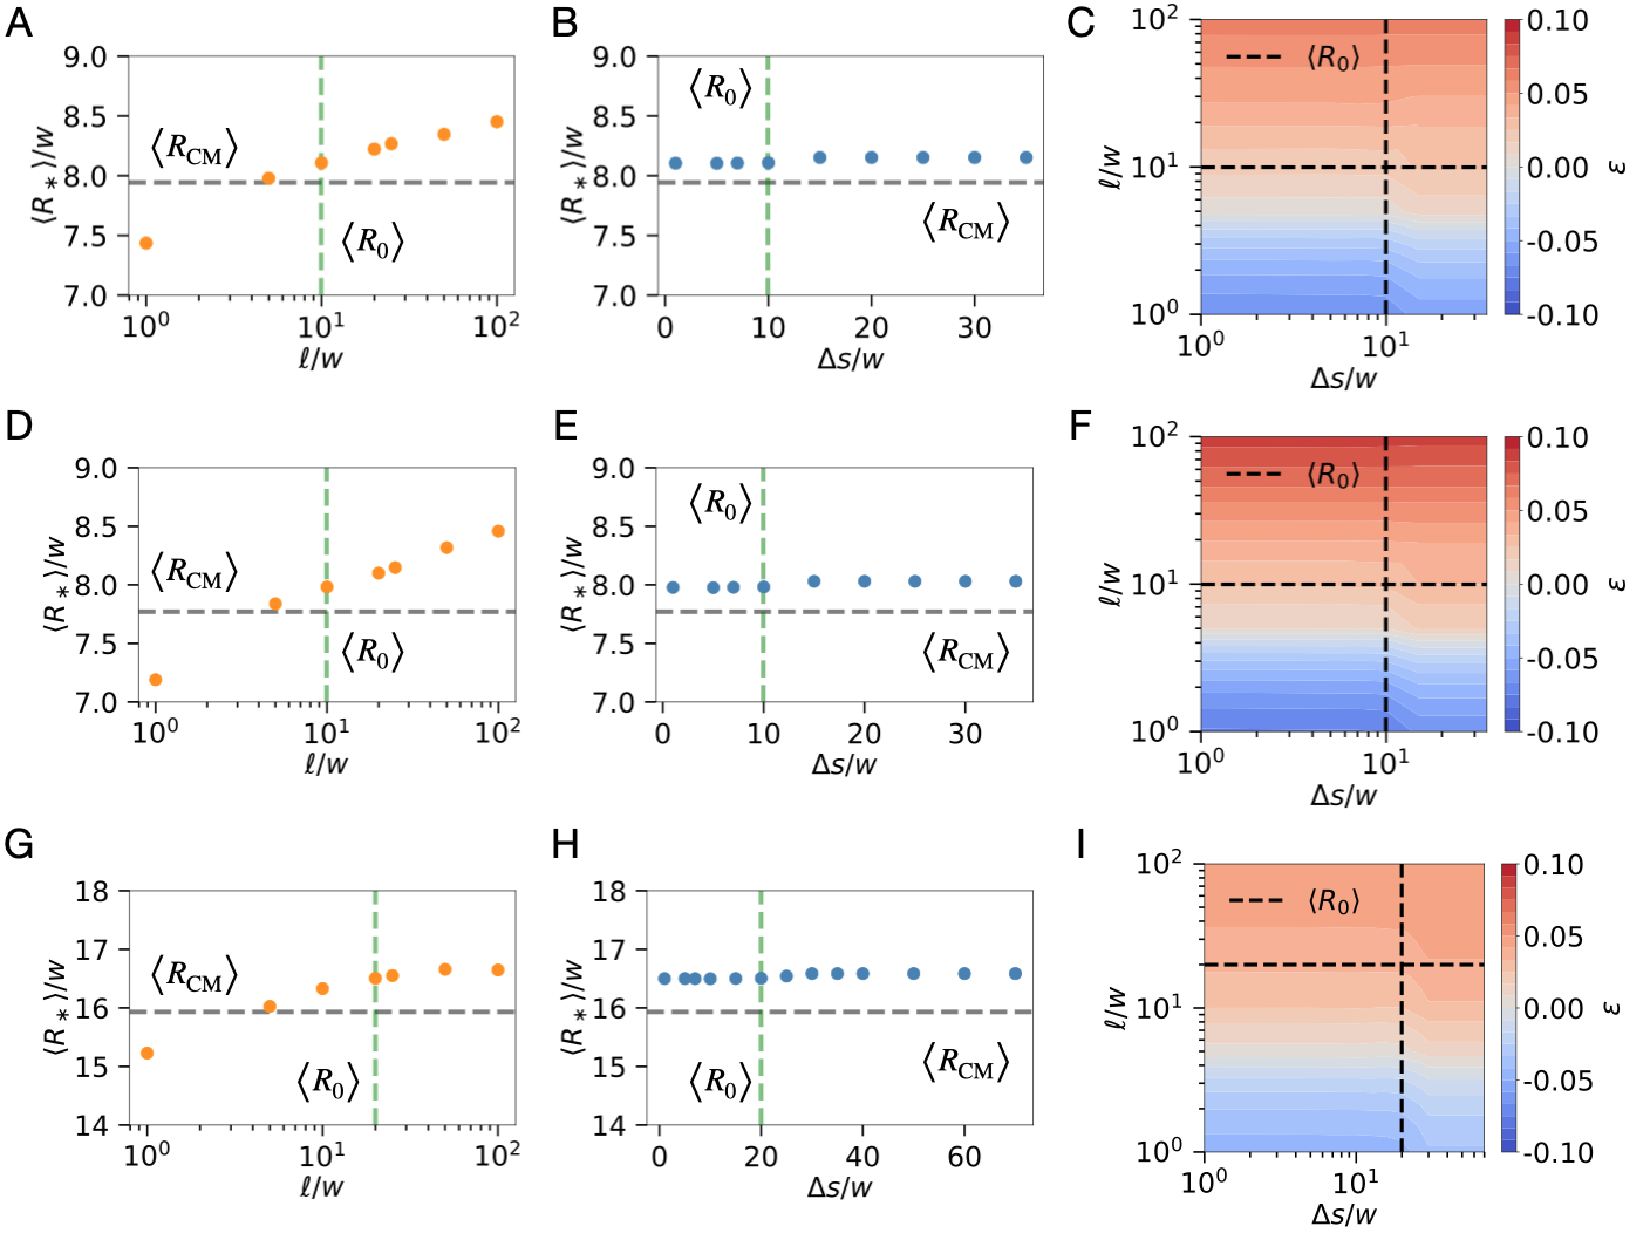
\includegraphics[scale=0.58]{MainContent/Figures/robustness_test_case.pdf}
\caption{\textbf{Effect of shell thickness $\ell$ and sector size $\ds$ on simulations of a passive droplet pair.}
\mbox{(A-C)} show simulations for the droplet pair when $[R_0, S_\mathrm{d}] = [10w, 40w]$.
(A) Mean droplet size $\langle R_\ast \rangle$ from the effective droplet model as a function of $\ell$ (orange dots) for $\dx \approx \ds \approx R_0$ compared to the ground truth $\mean{R_\mathrm{CM}}$ (gray dashed line) obtained from the continuous model.
The choice $\ell \approx R_0$ (green dashed line) provides good agreement and the error between $\left \langle R_\mathrm{CM} \right \rangle$ (dashed grey line) and $\left \langle R_\ast \right \rangle$ is less than $\pm 5\%$.
(B) $\langle R_\ast \rangle$ as a function of $\ds$ (blue dots) for $\dx \approx \ell \approx R_0$ compared to $\mean{R_\mathrm{CM}}$, where the error between $\left \langle R_\mathrm{CM} \right \rangle$ (dashed grey line) and $\left \langle R_\ast \right \rangle$ is less than $\pm 5\%$.
(C) Colorbar shows the error between the continuous model and the effective droplet model $\epsilon = [\langle R_\ast \rangle - \mean{R_\mathrm{CM}}] / \mean{R_\mathrm{CM}}$ is less than $\pm5\%$ for $\ds \approx \ell \approx R_0$.
\mbox{(D-F)} show simulations for the droplet pair when $[R_0, S_\mathrm{d}] = [10w, 100w]$.
\mbox{(G-I)} show simulations for the droplet pair when $[R_0, S_\mathrm{d}] = [20w, 80w]$.
We thus conclude that $\dx \approx \ds \approx \ell \approx R_0$ is the optimum choice for the simulation parameters for the effective droplet model. 
Remaining parameters are specified in Fig. \ref{fig:droplet_pair_schematics}.
}
\label{fig:robustness_test_case}
\end{figure}
Thus, from all the three different systems: $[R_0, S_\mathrm{d}] = [10w, 40w], [10w, 100w]$ and $[20w, 80w]$, we see that $\dx \approx \ds \approx \ell \approx R_0$ is a reasonable choice for the effective droplet model for which the error $\epsilon$ between the continuous model and the effective droplet model is less than $\pm 5\%$.

%%%%%%%%%%%%%%%%%%%%%%%%%%%%%%

\chapter{Droplet dynamics in external gradients in two dimensional systems}

\label{sec:droplet_gradient_2D}

Primarily, studies of phase separated condensates have mostly focused on three dimensional droplets. 
However, two dimensional phase separation is also relevant, for example, aggregation of shape regulating proteins; see Ref. \cite{gov2018} and emulsions in two dimensions; see Refs. \cite{Zwicker2015,Review2019,Bressloff_2020,Bressloff2020}.

We aim to demonstrate the effective model for a passive droplet in the presence of an external volume fraction gradient in two dimensional systems.
We compare the simulations using the effective droplet model with the continuous model and analytical predictions. 
Similar to a passive droplet in an external gradient in a three dimensional system; see Chapter \ref{chap:Chapter_5}, we first derive the droplet growth rate and drift speed for a passive droplet in an external volume fraction gradient in a large 2 dimensional system.

Consider an isolated passive droplet of radius $R \gg w$ with a polar co-ordinate
system centred at the droplet position $\vec{x_0}$.
The volume fraction outside the droplet can thus be expressed as $\phiOut(r, \theta)$, where $\theta \in [0, 2\pi]$. 
For simplicity, we again assume that the droplet experiences a one dimensional gradient that varies along the $x$-coordinate without loss of generality.
We utilize the framework of thin interface approximation and solve for the volume fraction profiles $\phiIn,~\phiOut$ inside and outside the droplet.
Since $\phiIn$ inside the droplet typically varies only a little, we use the thin-interface approximation and solve for $\phiIn$ from the steady state of \Eqref{eqn:RD_droplet_passive} using the boundary conditions $\phiIn(R) = \phiEqIn$ and $\partial_r \phiIn (0) = 0$ to obtain $\phiIn(r) = \phiEqIn$.

Similar to inside the droplet, the volume fraction inside in the background field $\phiOut$ also typically varies little can be solved from \Eqref{eqn:RD_droplet_passive} using the boundary conditions $\phi_\mathrm{out}(R) = \phiEq_\mathrm{out}$ and far from the droplet $\phi_\mathrm{out}(L) = \phi_{\infty} = \alpha + \beta \, L \, \text{cos}\,\theta$, where $L$ is the size of the large domain.
Note that since the volume fraction around the droplet varies as $\log(R)$, we do not consider truly infinite systems, but a large finite system of size $L$.
We thus obtain the volume fraction profile as 
\begin{equation*}
\phiOut(r, \theta) = \frac{\alpha - \frac {\phiEqOut \log(L) } { \log(R)}} { 1 - \frac{\log(L)}{\log(R)} } + \frac{\left ( \phiEqOut - \frac{\alpha - \frac {\phiEqOut \log(L) } {\log(R)}} { 1 - \frac{\log(L)}{\log(R)} } \right ) \log(r)}{\log(R)} + \left (\beta r - \frac{R^2 \beta}{r} \right ) \cos(\theta).
\end{equation*}
We now evaluate the local fluxes at the droplet surface similar to the approach used earlier as $\jIn = 0$,
\begin{equation*}
    \jOut \cdot \vec{n}= -D \left( 2 \beta \cos(\theta) +\frac{\left ( \phiEqOut - \frac{\alpha - \frac {\phiEqOut \log(L) } {\log(R)}} { 1 - \frac{\log(L)}{\log(R)} } \right )}{R \log R} \right ), 
\end{equation*}
and calculate the interfacial speed $v_n$ from \Eqref{eqn:InterfacialSpeed}.
We finally arrive at the droplet growth and drift speed from \Eqref{eqn:DropletGrowth} and \Eqref{eqn:DropletDrift} as

\begin{subequations}
\label{eqn:interfacefluxes_gradient_2D}
\begin{align}
	\frac{\mathrm{d} R}{\mathrm{d} t} &= \frac{1}{2 \pi} \int_{\Omega} D \left( 2 \beta \cos(\theta) +\frac{\left ( \phiEqOut - \frac{\alpha - \frac {\phiEqOut \log(L) } { \log(R)}} { 1 - \frac{\log(L)}{\log(R)} } \right )}{R \log R} \right ) \mathrm{d}A = \frac{D (\alpha - \phiEqOut)}{R \log \frac{L}{R}}
	\text{~and}
    \\[10pt]
    \frac{\mathrm{d} x_0}{\mathrm{d} t} &= \frac{1}{\pi} \int_{\Omega} D \left( 2 \beta \cos(\theta) +\frac{\left ( \phiEqOut - \frac{\alpha - \frac {\phiEqOut \log(L) } {\log(R)}} { 1 - \frac{\log(L)}{\log(R)} } \right )}{R \log R} \right ) \cos(\theta) \, \mathrm{d}A = 2 D \beta,
\end{align}
\end{subequations}
where $D$ is the diffusivity, $L$ is the system size, $R$ is the droplet radius, $\Omega$ is the droplet surface and $\mathrm{d} A$ is the area element on the droplet surface.

\begin{figure}[t]
\centering
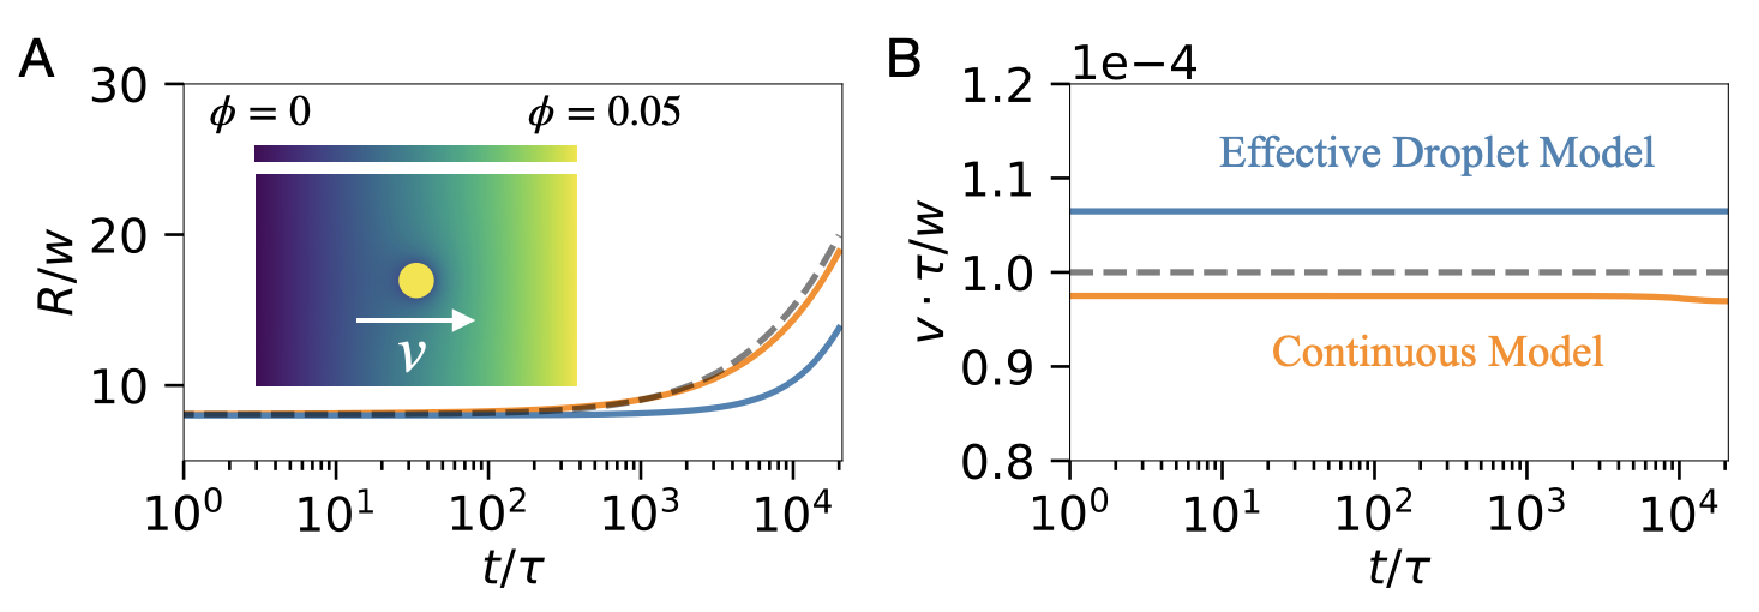
\includegraphics[scale=0.5]{MainContent/Figures/Strong_Gradient_2D.pdf}
\caption{\textbf{Droplet dynamics in external gradients in two dimensional systems.}
(A) Droplet radius $R$ as a function of time $t$ from the effective droplet model (blue), analytical prediction (dashed line) from \Eqsref{eqn:interfacefluxes_gradient_2D} and the continuous model (orange).
The inset shows a schematic of the simulation with the imposed gradient of droplet material.
(B) Droplet drift speed $v$ as function of $t$ using the effective droplet model (blue) and the analytical prediction (dashed line) from \Eqsref{eqn:interfacefluxes_gradient_2D}, with simulations using the continuous model (orange).
\mbox{(A, B)}
The continuous and the effective droplet model uses a Cartesian 2 dimensional domain with $x,y \in [-L, L]$, with $L=500 w$. The boundary conditions are $\mu(x=-L) = 0$ and $\mu(x=L)= 0.0427\,b\,w^2$ for the continuous model and $\phiOut(x=-L) = 0$ and $\phiOut(x=L)= 0.05$ to maintain the gradient throughout the system.
The effective model uses $\dx \approx \ell \approx \Delta s \approx R_0$.
Note that in the absence of droplets, boundary conditions imply identical linear gradient in the effective droplet model as $\phi=\phi(x)$ and in the continuous model as $\phiOut=\phiOut(x)$, which were also used to initialize the background for both the models.
Remaining parameters are specified in Fig. \ref{fig:droplet_pair_schematics}.
}
\label{fig:drop_in_gradient_2D}
\end{figure}

We simulate a single passive droplet of initial radius $R_0 = 6w$ immersed in a linear volume fraction gradient of the droplet material. 
Similar to the case of the passive droplet growing in a supersaturated medium, the passive droplet in this case also grows over time by taking material from the surroundings. 
Furthermore, as $\jOut \cdot \vec{n}$ has an angular dependence, it results in unequal fluxes leading to droplet drift along the gradient.
The continuous and the effective droplet model use a Cartesian two dimensional domain with $x,y \in [-L, L]$, with $L=500 w$. 
The boundary conditions are $\mu(x=-L) = 0$ and $\mu(x=L)= 0.0427\,b\,w^3$ for the continuous model and $\phiOut(x=-L) = 0$ and $\phiOut(x=L)= 0.05$ to maintain the gradient throughout the system.
The effective model uses $\dx \approx \ell \approx \Delta s \approx R_0$.
\figref{fig:drop_in_gradient_2D} shows droplet growth and drift speed using the effective droplet model with optimum parameters ($\dx \approx \ell \approx \Delta s \approx R_0$), simulations using the continuous model and analytical predictions from \Eqsref{eqn:interfacefluxes_gradient_2D}.

%%%%%%%%%%%%%%%%%%%%%%%%%%%%%%%%

\end{appendices}